\documentclass[tikz,border=15pt]{standalone}
\usepackage{circuitikz}
\usepackage{amsmath}
\begin{document}
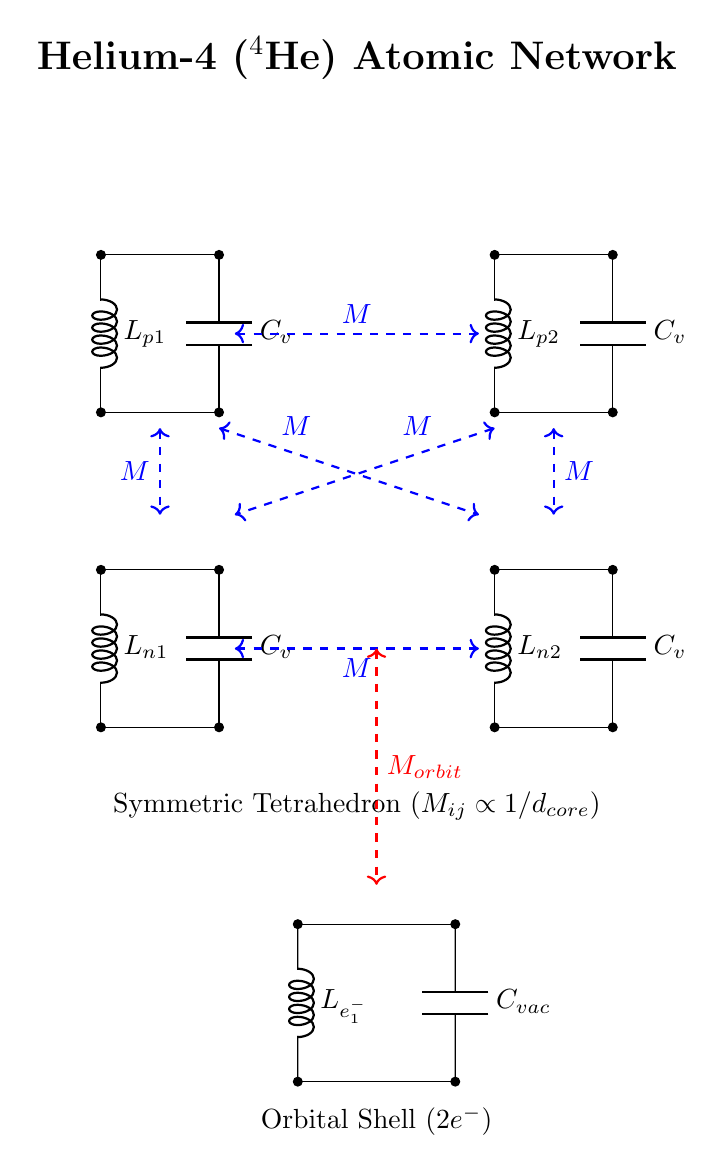
\begin{tikzpicture}
    \def\tank#1#2#3{
        \begin{scope}[shift={(#1)}]
            \draw (0,0.5) to[L=$#3$, *-*] (0,-1.5);
            \draw (1.5,0.5) to[C=$C_v$, *-*] (1.5,-1.5);
            \draw (0,0.5) -- (1.5,0.5);
            \draw (0,-1.5) -- (1.5,-1.5);
        \end{scope}
    }
    
    \tank{0,4}{1}{L_{p1}}
    \tank{5,4}{2}{L_{p2}}
    \tank{0,0}{3}{L_{n1}}
    \tank{5,0}{4}{L_{n2}}
    
    % Orbital Electrons (Far-Field Displacement Tanks)
    \draw (2.5, -4) to[L=$L_{e_1^-}$, *-*] (2.5,-6);
    \draw (4.5, -4) to[C=$C_{vac}$, *-*] (4.5,-6);
    \draw (2.5,-4) -- (4.5,-4);
    \draw (2.5,-6) -- (4.5,-6);
    \node at (3.5, -6.5) {Orbital Shell ($2e^-$)};
    
    % Core Mutual Coupling
    \draw[<->, dashed, blue, thick] (1.7,3.5) -- (4.8,3.5) node[midway, above] {$M$};
    \draw[<->, dashed, blue, thick] (1.7,-0.5) -- (4.8,-0.5) node[midway, below] {$M$};
    \draw[<->, dashed, blue, thick] (0.75,2.3) -- (0.75,1.2) node[midway, left] {$M$};
    \draw[<->, dashed, blue, thick] (5.75,2.3) -- (5.75,1.2) node[midway, right] {$M$};
    \draw[<->, dashed, blue, thick] (1.5,2.3) -- (4.8,1.2) node[midway, above right, pos=0.2] {$M$};
    \draw[<->, dashed, blue, thick] (5,2.3) -- (1.7,1.2) node[midway, above left, pos=0.2] {$M$};
    
    % Orbit Coupling
    \draw[<->, dashed, red, thick] (3.5,-0.5) -- (3.5,-3.5) node[midway, right] {$M_{orbit}$};
    
    \node at (3.25, 7.0) {\Large \textbf{Helium-4 ($^4\text{He}$) Atomic Network}};
    \node at (3.25, -2.5) {Symmetric Tetrahedron ($M_{ij} \propto 1/d_{core}$)};
\end{tikzpicture}
\end{document}
